\section{Incorporating other detector prototypes into ProtoDUNE-ND}
\label{sec:MINERvA_MINOS}

\begin{figure}[htb]
	\centering
	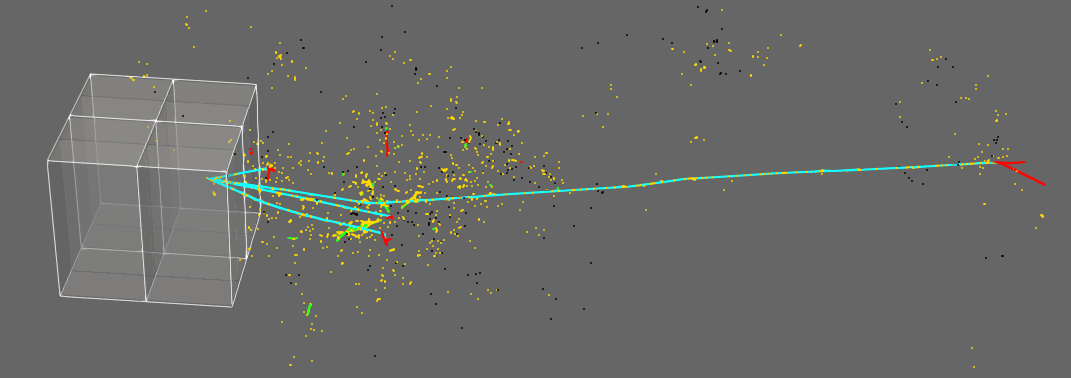
\includegraphics[width=0.8\textwidth]{{plots/EventDisplays/8.17GeV_rectangle_crop}.png}
	\caption{Example ArgonBox simulated event for an 8.17 GeV $\nu_{\mu}$--argon neutral-current multi-pion interaction, in which the pions are not contained in the module. Energy deposits in a bulk volume of LAr are color-coded according to the particle type: $\pi^{\pm}$ --- blue; $\mu^{\pm}$ --- purple; $e^{+}$ --- green; $e^{-}$ --- yellow; proton --- red; recoiling nuclei --- black. The event vertex was randomly placed inside the active volume of the ArgonCube 2x2 Demonstrator, the geometry for which is superimposed on these images, but which is not simulated by ArgonBox.}
	\label{fig:leaky_event}
\end{figure}
Given the ArgonCube 2x2 Demonstrator's size and the relatively high energy NuMI ME beam, many events will not be contained in the 2x2 alone. Figure~\ref{fig:leaky_event} shows a neutral current event where many pions are produced, but in which the pions and subsequent hadronic showers extend far beyond the detector. Indeed, many such events would not be contained in the full ArgoNCube deployment at the DUNE ND, in the LBNF beamline, and for charged-current events, the muon will be uncontained most of the time. For this reason, and because it is not possible to magnetize the large LAr component, further, magnetized, tracking detectors are proposed downstream of ArgonCube in the full DUNE ND complex, and the requirement to tag side-escaping particles is discussed in Ref.~\cite{dune_ndcsg}. Broadly speaking, three additional subdetector options are considered for the DUNE-ND design, in addition to ArgonCube~\cite{dune_ndcsg}, as introduced in Section~\ref{sec:tracking_detectors}: a scintillator tracking detector; a magnetized low-density tracking detector; and a Cosmic Ray Tagging (CRT) system.

Prototypes for these detectors are currently being planned, and the ProtoDUNE-ND complex is intended to evolve over time to accommodate them. As has been remarked, the cryogenic system for the ArgonCube 2x2 will be moveable to test key components of the DUNE-PRISM technical design, which will allow ProtoDUNE-ND to be easily reconfigured to accommodate any future prototype detectors. In this section, we discuss how adding those additional detectors will enhance the neutrino engineering studies possible with ProtoDUNE-ND. In this section, we broadly consider the additional detector physics studies that would be possible should prototypes for the other subdetector options become available. With multiple subdetectors included in ProtoDUNE-ND, multi-detector reconstruction capabilities can be developed and tested. Additionally, if the sign and momentum of escaping hadrons and muons can be measured, it may be possible to make physics measurements with ProtoDUNE-ND, which would be beneficial to the overall DUNE program, although that discussion is beyond the scope of this document.

\subsection{Scintillator detector}
\label{sec:minerva}
All DUNE ND designs considered in Ref.~\cite{dune_ndcsg} include some fast scintillator component, either the large fully activeThree-Dimensional Scintillator Tracker (3DST), downstream of the LAr ArgonCube component, and scintillator components downstream of the HPgTPC to tag escaping neutral particles. There is a significant reconstruction challenge in matching the escaping tracks from the LAr component, with the signals in the scintillator, given the slow charge readout in the LAr TPC, and the high multiplicity DUNE-ND environment. As such, a test of track matching between LAr and any scintillator detector would be a valuable way to develop and test reconstruction software for the DUNE ND.

\subsubsection{Acceptance}
As discussed in Section~\ref{sec:detector-physics-studies}, a large fraction of particles will not be contained in the 2x2 alone. A downstream scintillator detector would recover many of these particles, and would make it possible to benchmark the 2x2 response to a wider range of particle energies, and therefore the expected DUNE phase-space. As discussed previously in this note, the 2x2 module will not be placed in a test beam prior to installation in the NuMI beam at Fermilab, therefore measurements in which the energy scale of the 2x2 can be calibrated will be vital to assess the quality of energy reconstruction in the detector. In particular, the $\pi^{0}$ mass-peak reconstruction test described in Section~\ref{sec:pi0_reco} would benefit from wider acceptance, and if the energy of escaping charged particles could be reconstructed in the scintillator detector, the response to charged particles of a known energy could be characterized.

\subsubsection{Neutron tagging}
The ability to identify and measure neutrons produced in neutrino interactions is of great interest to DUNE.  At the far detector recoil protons can be identified and easily associated to the neutrino interaction.  However, at the near detector, confusion due to multiple neutrino interactions in the same beam spill poses a unique challenge.  As discussed in Section~\ref{sec:2x2_neutron}, a key detector physics goal of ProtoDUNE-ND is to determine whether neutron-induced proton recoils can be identified in a LAr TPC, specifically in ArgonCube. Because neutrons can travel $\mathcal{O}\left(1\right)\,\mathrm{m}$ in LAr without interacting, and proton recoils from fast neutrons typically deposit energy on a single pixel and thus contain no directionality, event association is not possible without matching the charge deposit to an ArCLight optical flash with fast timing resolution.
 
Additionally, it may be possible to measure the neutron energy from time-of-flight in the DUNE ND using the ECAL with very fast, sub-nanosecond timing resolution. This will require matching muon tracks from either the LAr or HPgTPCs to hits in the ECAL in order to reconstruct the neutrino interaction vertex time with high precision, and also identify and timestamp a subsequent neutron interaction in the scintillator tiles of the ECAL. This would give the DUNE ND unprecedented ability to make measurements of the neutron energy spectrum in neutrino-argon interactions. This technique has not been tested in a high-rate environment. Because the neutrons may propagate for $\mathcal{O}\left(10\right)\,\mathrm{ns}$, even a very fast detector may suffer from confusion due to pile-up. The ability to match both muons and neutrons originating in LAr to a fast-timing scintillator detector would be a direct test of the feasibility of this technique in DUNE ND. This has profound impact on the design of the ECAL, which would need to be optimized for both EM and neutron reconstruction if this technique is demonstrated to be viable.
 
\subsection{Magnetized low-density tracking detector}
The DUNE ND will employ a high-pressure argon gas TPC (HPgTPC) which will operate inside a magnetic field, downstream of the LAr component. As well as providing a target to sample low threshold, high resolution, argon interactions, it will act as a downstream tracker for particles exiting the LAr (and possible 3DST) detectors, and will provide sign and momentum measurements of particles in the magnetic field. A prototype HPgTPC is currently being planned, although the details are not available for a sophisticated study at this time.

\subsubsection{Acceptance}
As when including a scintillator tracking detector downstream of the ArgonCube 2x2 Demonstrator in ProtoDUNE-ND, including an HPgTPC prototype would improve the acceptance of charged particles produced in the LAr volume, as it would be possible to make momentum measurements by curvature in the magnetic field. Unlike a scintillator tracker, the HPgTPC prototype would be unable to improve acceptance of neutral particles, but could be coupled with a downstream ECal, as indeed the HPgTPC is in the DUNE ND design. Assuming the HPgTPC prototype will also be magnetized, it has the potential to improve acceptance to higher momentum forward particles than with a downstream scintillator tracker, where containment by range might be limited. Of course, which has greater acceptance depends on the size and strength of the HPgTPC prototype magnet, and the size of a downstream tracking scintillator detector, but either would improve the acceptance relative to the 2x2-only case.

\subsubsection{Multiple-coulomb scattering (MCS)}
For many DUNE far detector (FD) events, the muon will be contained in the FD module, and the muon momentum will be measured by range. For high-angle muon events, where the muon will not be contained, multiple-coulomb scattering (MCS) will be used. Similarly, the DUNE ND will have a magnetized downstream tracking detector to measure forward, high-energy muons by curvature, but high angle muons will not be reconstructed in the tracker. In order to cover the phase-space sampled at the FD, it also needs to be shown that MCS measurements can also be made in the segmented ArgonCube TPC.

Such measurements have been carried out in a LAr TPC by MicroBooNE~\cite{Abratenko:2017nki}, although the momentum range is somewhat limited as the only validation sample available is composed of muons which stop in the detector, for which a momentum by range measurement can be made. However, such measurements may be more challenging in a modular TPC such as ArgonCube, where tracks are necessarily broken into segments which are read out separately, and then combined in downstream software. Although there are only four modules in the ArgonCube 2x2 Demonstrator, each is split into two TPCs, so tracks which exit the downstream face of the 2x2 module may be sampled by up to four independent charge readout planes. With a downstream detector capable of making a precise muon momentum measurement, it would be possible to demonstrate that multiple coulomb scattering will be a viable technique for making momentum measurements in the full ArgonCube deployment in the DUNE ND.

Furthermore, a major outstanding DUNE ND design question is whether both the LAr component and the downstream tracker need to be moved off-axis for DUNE-PRISM, or whether the LAr component alone can be moved, which hinges on how well the muon momentum can be reconstructed through MCS alone.

\subsection{Cosmic Ray Tagger (CRT)}
A key design choice for the DUNE ND is whether or not a muon tagging system is required --- for example, a series of scintillator planes surrounding the LAr TPC, as for SBND and MicroBooNE~\cite{CRT} --- to tag side-escaping muons, or to tag entering particles, either cosmic muons, or particles from beam-induced events in the surrounding rock. ProtoDUNE-ND provides an opportunity to test how well ArgonCube modules can tag such particles and separate them from beam neutrino events in the fiducial volume, either using timing, or by tagging particles which enter or exit a readout or ArCLight plane, and inform the decision on whether the full DUNE DN requires a CRT system.

\subsubsection{Space charge and electric field uniformity}
\label{sec:efield}
One concern for LAr detectors in a high intensity beam is the build up of space charge --- long-lived argon ions which drift slowly towards the cathode --- and possible affects on the uniformity of the electric field which may accumulate over time. In currently operating and near-future LAr detectors~\cite{Ereditato:2014lra, Antonello:2015lea}, both cosmic tracks and UV lasers are used to calibrate for distortions in the electric field. Both the UV laser track and high energy cosmic muons are expected to leave straight tracks in the detector. If the drift field is not uniform across the detector, ionization electrons produced along the length of this track will not drift at the same speed, or with a constant direction, and will result in a distorted track at the readout plane. By comparing the reconstructed and expected track, a map of the electric field distortion can be built up for calibration purposes.

Assuming that the ArgonCube 2x2 Demonstrator is equipped with scintillator panels to tag cosmic tracks using a timing coincidence between two sides of the detector, and reasonable spatial resolution on those scintillator paddles, electric field distortions could be measured in the 2x2 Demonstrator module. By looking at beam-on, and beam-off data, it would be possible to look at the possible affect of space charge build-up over time due to the high event rate in the NuMI beam. If significant space charge build-up were observed, this would inform the future ArgonCube design for the DUNE ND, as a higher drift field strength would be required.

Additionally, although the electric-field uniformity of the resistive field shell will be checked in a small scale LAr TPC at Bern, a check of the electric-field uniformity and stability over time for full-size ArgonCube modules would be a valuable final validation of the design.

\subsubsection{Cosmic and rock muon suppression}
\label{sec:cosmic-suppression}

The DUNE ND is located underground with a \SI{50}{\metre} overburden, that reduces the cosmic flux by orders of magnitude compared to surface detectors. The cosmic rate in MINERvA (currently in the MINOS ND hall where ProtoDUNE-ND will be sited) is \SI{18}{\hertz}, for $\sim$\SI{6}{\metre\squared}. For the ArgonCube 2x2, in the $\sim$\SI{150}{\micro\second} readout window, assuming $\sim$\SI{2}{\metre\squared}, the rate of cosmics muons is 0.001 per readout window. Reading out around spills only, will result in a coincident cosmic muon once every 20 minutes.
In DUNE ND we expect $\sim$10 rock muons per spill, which will be on average $\sim$\SI{1}{\micro\second} apart in time. They are unlikely to overlap any neutrino activity in 3D, but the fast timing will provide an additional handle.

By using a CRT system to tag cosmic or rock events using a timing coincidence, methods for rejecting them can be validated independently. For example, we expect that the good timing resolution and light localization from ArcLight will allow cosmics out of the beam window to be rejected with a high efficiency. Additionally, if a cosmic muon traverses a pixel plane, or an ArcLight plane, we would expect to see a large charge deposition or a large number of photoelectrons measured, which could be an additional way to reject cosmic muons. Both of these methods can be validated with ProtoDUNE-ND.

\subsubsection{Acceptance}
As the ArgonCube 2x2 Demonstrator is a fraction of the full DUNE ND ArgonCube deployment, many more particles will escape the sides of the detector. An independent CRT system provides an exellent opportunity to test how well ArgonCube modules can tag exiting particles, and will ensure that we are able to select contained tracks and showers with high confidence. This will be valuable for benchmarking the energy response with the $\pi^{0}$ mass peak study described in Section~\ref{sec:pi0_reco}, and for any other energy response studies which will have to rely on contained tracks. Depending on the design of the CRT system, it may be possible to increase the phase space of the contained events, as the CRTs will capture some of the energy that would otherwise be uncontained.
